\documentclass{ximera}

\usepackage{gensymb}
\usepackage{tabularx}
\usepackage{mdframed}
\usepackage{pdfpages}
%\usepackage{chngcntr}

\let\problem\relax
\let\endproblem\relax

\newcommand{\property}[2]{#1#2}




\newtheoremstyle{SlantTheorem}{\topsep}{\fill}%%% space between body and thm
 {\slshape}                      %%% Thm body font
 {}                              %%% Indent amount (empty = no indent)
 {\bfseries\sffamily}            %%% Thm head font
 {}                              %%% Punctuation after thm head
 {3ex}                           %%% Space after thm head
 {\thmname{#1}\thmnumber{ #2}\thmnote{ \bfseries(#3)}} %%% Thm head spec
\theoremstyle{SlantTheorem}
\newtheorem{problem}{Problem}[]

%\counterwithin*{problem}{section}



%%%%%%%%%%%%%%%%%%%%%%%%%%%%Jenny's code%%%%%%%%%%%%%%%%%%%%

%%% Solution environment
%\newenvironment{solution}{
%\ifhandout\setbox0\vbox\bgroup\else
%\begin{trivlist}\item[\hskip \labelsep\small\itshape\bfseries Solution\hspace{2ex}]
%\par\noindent\upshape\small
%\fi}
%{\ifhandout\egroup\else
%\end{trivlist}
%\fi}
%
%
%%% instructorIntro environment
%\ifhandout
%\newenvironment{instructorIntro}[1][false]%
%{%
%\def\givenatend{\boolean{#1}}\ifthenelse{\boolean{#1}}{\begin{trivlist}\item}{\setbox0\vbox\bgroup}{}
%}
%{%
%\ifthenelse{\givenatend}{\end{trivlist}}{\egroup}{}
%}
%\else
%\newenvironment{instructorIntro}[1][false]%
%{%
%  \ifthenelse{\boolean{#1}}{\begin{trivlist}\item[\hskip \labelsep\bfseries Instructor Notes:\hspace{2ex}]}
%{\begin{trivlist}\item[\hskip \labelsep\bfseries Instructor Notes:\hspace{2ex}]}
%{}
%}
%% %% line at the bottom} 
%{\end{trivlist}\par\addvspace{.5ex}\nobreak\noindent\hung} 
%\fi
%
%


\let\instructorNotes\relax
\let\endinstructorNotes\relax
%%% instructorNotes environment
\ifhandout
\newenvironment{instructorNotes}[1][false]%
{%
\def\givenatend{\boolean{#1}}\ifthenelse{\boolean{#1}}{\begin{trivlist}\item}{\setbox0\vbox\bgroup}{}
}
{%
\ifthenelse{\givenatend}{\end{trivlist}}{\egroup}{}
}
\else
\newenvironment{instructorNotes}[1][false]%
{%
  \ifthenelse{\boolean{#1}}{\begin{trivlist}\item[\hskip \labelsep\bfseries {\Large Instructor Notes: \\} \hspace{\textwidth} ]}
{\begin{trivlist}\item[\hskip \labelsep\bfseries {\Large Instructor Notes: \\} \hspace{\textwidth} ]}
{}
}
{\end{trivlist}}
\fi


%% Suggested Timing
\newcommand{\timing}[1]{{\bf Suggested Timing: \hspace{2ex}} #1}




\hypersetup{
    colorlinks=true,       % false: boxed links; true: colored links
    linkcolor=blue,          % color of internal links (change box color with linkbordercolor)
    citecolor=green,        % color of links to bibliography
    filecolor=magenta,      % color of file links
    urlcolor=cyan           % color of external links
}

\title{Measuring Length, Area, and Volume}
\author{Jenny Sheldon}

\begin{document}

\begin{abstract}
We talk about how to measure.
\end{abstract}
\maketitle

Now that we've talked about what measurement gives us and how to think about units of measure, we're ready to do some measuring. Quite a bit of this content is related to the ideas of dimension, so it's a good idea to refresh yourself on that content by re-reading the section or looking back over your notes again before moving forward.

We should start by talking about what we mean by length, area, and volume.
\begin{definition}
The \dfn{length} of an object is the amount of one-dimensional space the object takes up.
\end{definition}
\begin{definition}
The \dfn{area} of an object is the amount of two-dimensional space the object takes up.
\end{definition}
\begin{definition}
The \dfn{volume} of an object is the amount of three-dimensional space the object takes up.
\end{definition}
I hope you are seeing a pattern here -- so much so that perhaps you could even define an analog of volume in four-dimensional space (but don't worry, we won't work with that here). Keep looking for patterns as we start measuring these things. Where can you find similarities between length, area, and volume? Where do you find differences? Keep good notes on your thoughts. Also, pause and notice that the meaning of length, area, or volume doesn't have anything to do with which unit we use to measure, or with any specific formula. These are general meanings that we will continue to explore for several sections.

\section{The process of measurement}
We will think about measuring length, area, or volume as a four step process.
\begin{enumerate}[label=\arabic{enumi}.]
	\item Choose an aspect to measure and describe it specifically.
	\item Choose an appropriate unit for measuring and describe it specifically.
	\item Iterate your unit all over the object, leaving no gaps and no overlaps.
	\item Report and interpret your results.
\end{enumerate}

We discussed the first two steps here in the previous section. Remember that describing things specifically is key to making a good measurement, and your descriptions should make it clear what dimension you're working in. Also remember that an appropriate unit is one that is the same dimension as the aspect you are measuring.

The word ``iterate'' in step 3 might feel a little strange here, but the goal is to again see that the process of measuring is the same for length, area, or volume. If we are measuring length, we might say ``line up the unit end-to-end'' instead of saying ``iterate''. If we are measuring area, we might say ``cover the object with the unit'' instead of using ``iterate''. And if we are measuring volume, we might say ``fill the object with units'' instead of talking about iterating. Please use vocabulary that makes sense to you and to the situation!

\begin{example}
In the previous section, we talked about measuring a golf club using a golf pencil. Let's return to this example to talk about how we would actually make this measurement.

First, we choose an aspect to measure. In this case it's the \wordChoice{\choice[correct]{length} \choice{area} \choice{volume}} of the golf club. We could also draw a picture of the golf club and indicate on our picture what we mean by the length to make things even more clear.
\begin{image}
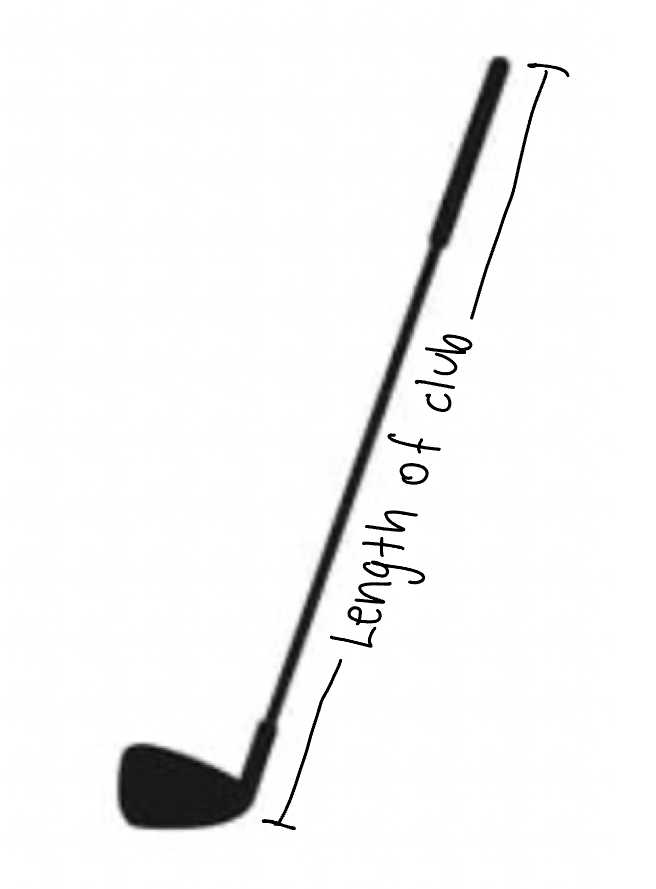
\includegraphics[width=0.3\textwidth]{Club.png}
\end{image}
Next, we choose a unit of measure. In this case it's the \wordChoice{\choice[correct]{length} \choice{area} \choice{volume}} of the golf pencil. We know this unit of measure is appropriate for this measurement because both the aspect we are measuring and the unit we are using are \wordChoice{\choice[correct]{1D} \choice{2D} \choice{3D}}. We could again draw and label a picture of our unit if we found that helpful, but we'll skip it for this example.

Our third step is to iterate the unit all over the object, leaving no gaps and no overlaps. In this case we want to cover up the entire length of the golf club with pencils. So, we start at one end of the golf club and line up our unit. We then line up the next unit with the end of the first unit, leaving no gaps and no overlaps. We keep using the same unit of measure, so we don't turn the pencil sideways. We keep repeating this process until we have accounted for the entire length of the golf club. We include a drawing of our process below.
\begin{image}
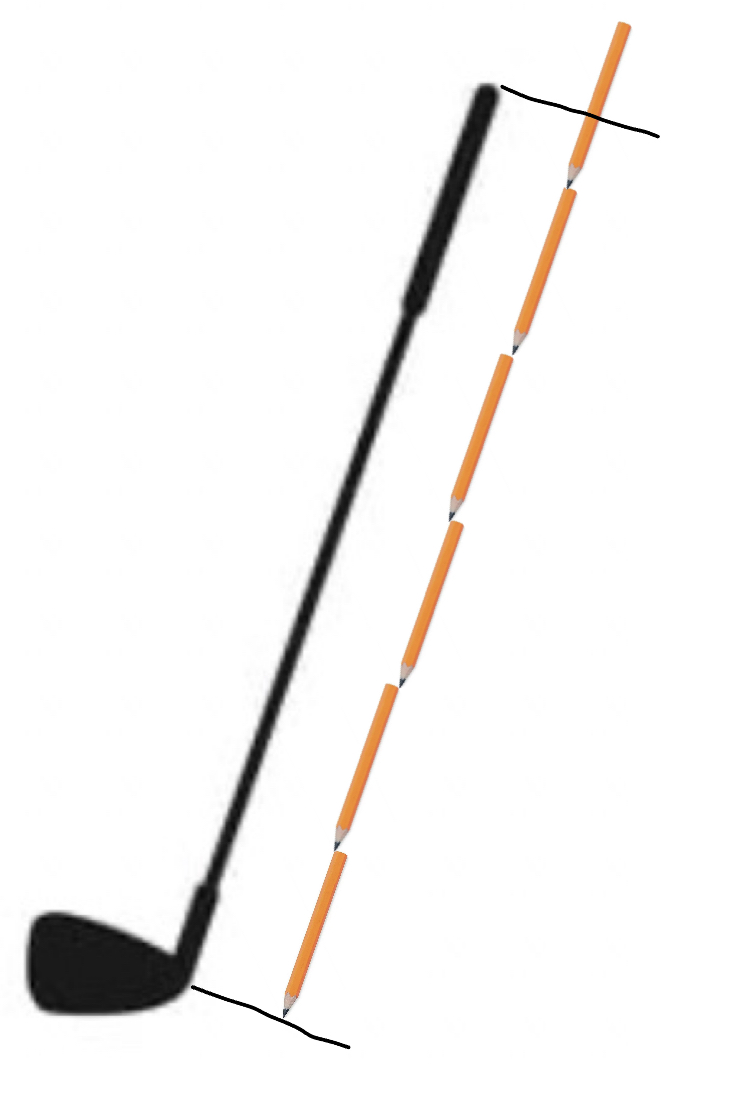
\includegraphics[width=0.3\textwidth]{MeasuredClub.png}
\end{image}
For our fourth step, we report and interpret our results. In this case it looks like we used $5\frac{1}{3}$ pencils to cover up the entire length of the golf club. To be really precise, we would have to make sure that last pencil is cut into three equal pieces! This means that our answer is that the length of the golf club is $\answer[given]{5+\frac{1}{3}}$ pencil lengths. Our answer means that if we think of the length of the pencil as one unit, the length of the golf club is $5 \frac13$ times as much as that original unit, or that it takes $5 \frac13$ copies of our unit to make up the 1D space that the length of the club takes up. Remember, that's what it means to be a length of something!

\end{example}

\begin{question}
Pause and think: how would the explanation above change if we were measuring an area? A volume?
\begin{freeResponse} Enter your thoughts here! \end{freeResponse}
\end{question}

\section{Approximate measurements}

Notice that in the previous section, we actually gave an approximate answer to the length example, because we estimated that the last pencil was about $\frac13$ of a full pencil's length. This is because in order to approximate length, area, or volume, we follow essentially the same four-step process for measurement that we do in order to get an exact measurement. The main difference is that when we approximate, it's okay to have gaps or overlaps, and it's okay to count too much or too little area. The closer we want our approximation to be, however, the less often we should leave those gaps, overlaps, or extra space.

\begin{example}
Estimate the area inside the shape below.
\begin{center}
\begin{tikzpicture}
\draw[gray, step=0.4] (0,0) grid (5,5);
\draw[smooth, very thick] plot coordinates {(0.5,0.5) (1,4) (3,3) (4,5) (5,2) (3,2) (2,1) (0.5,0.5)};
\end{tikzpicture}
\end{center}

For our process of measurement, we would like to measure the area inside the shape, and area is the amount of 2D space that the object takes up. Since the object is on top of a grid, we will use the area of one grid square as our unit. The area of the grid square is \wordChoice{\choice{1D} \choice[correct]{2D} \choice{3D}}, and so is the area we are trying to measure, so this unit is appropriate to use.

To estimate the area, the most basic thing we could do would be to count the number of grid squares inside the shape. To find an exact area, we would have to leave no gaps and no overlaps, but to estimate we don't have to be quite as precise. So, for instance, one strategy we could use would be to count only the squares that are fully inside the shape. I counted $45$ squares inside the shape. How many did you count? $\answer[tolerance=8]{45}$

We now report and interpret our answer. Since I counted $45$ squares inside the shape, I would answer that the shape's area is approximately $45$ squares. If you counted a different number, your answer would be different than mine, and that's perfectly fine in this case! My answer means that the amount of 2D space inside the shape is approximately the same as $45$ copies of the 2D space inside my unit. My estimate here is probably \wordChoice{\choice{an over estimate (too big)} \choice[correct]{an under estimate (too small)}} because I didn't account for all of the space inside the shape.
\end{example}

\begin{question}
Pause and think: there are many other ways to estimate the area of the shape in the previous example. Jot down at least two other strategies that you could use to make this estimate (and possibly get a different answer).
\begin{freeResponse} Your ideas go here! \end{freeResponse}
\end{question}

In the example above, we used the grid squares as our area unit, and grid squares are often convenient units to use. In fact, units that are square are so convenient, we give them a special name.
\begin{definition}
A \dfn{square unit} is a unit which is in the shape of a square. For instance, a \dfn{square inch} is a square whose sides measure 1 inch. A \dfn{square centimeter} is a square whose sides measure 1 centimeter. A \dfn{square mile} is a square whose sides measure 1 mile.
\end{definition}
However, we don't need to use square units to make our estimates. In fact, there's a game some people play where they try to estimate the number of candies in a jar. Usually the point of this game is that the person whose estimate is closest to the actual number of candies wins the whole jar. This game is really just about estimating the amount of 3D space inside the jar using the candies. 
\begin{image}
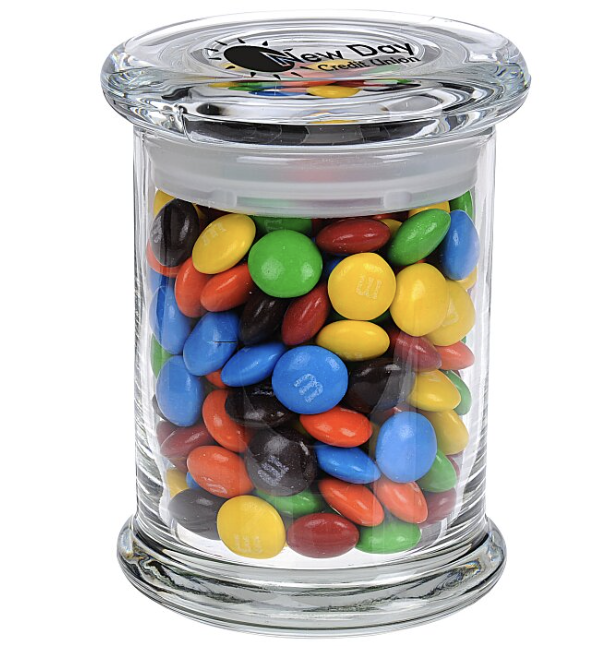
\includegraphics[width=0.3\textwidth]{CandyJar.png}
\end{image}
The amount of 3D space inside the jar is the aspect we are measuring, and one individual candy is our unit. We fill the jar with candies, and then the number of candies is an approximation for the 3D space inside the jar. The candies don't fill the jar exactly, since there is a bit of space between each one. These are the gaps that we don't want to leave for an exact measurement, but we are okay with for an approximation. In other words, the number of candies is \wordChoice{\choice{an over estimate (too big)} \choice[correct]{an under estimate (too small)}} for the exact volume because we don't account for all of the space inside the jar. So, if you ever run across this game after this, you can use your geometry approximation skills to win the candy!



\section{Moving and additivity}

As we begin to work with measuring, one of the first things we want to kids to recognize and use concerning length, area, and volume is that they are additive. We can write this down formally as follows.
\begin{definition}
The \dfn{additivity principle} says that if you take two lengths, areas, or volumes and put them together, you add together the length, area, or volume of each part to get the length, area, or volume of the whole.
\end{definition}

This should almost feel like common sense, but it's a powerful technique that we want kids to both use and recognize when they are using. So, in our explanations we'd like to point out when we are using this principle.

\begin{question}
Javier has a bucket that has $40$ cubic centimeters of sand in it, and Damien has a bucket that has $50$ cubic centimeters of sand in it. If the kids both dump their buckets of sand into a larger, empty bucket, how much sand will be in the larger bucket?

\begin{prompt} $\answer[given]{90}$ cubic centimeters of sand \end{prompt}

\begin{explanation}
Javier and Damien start out with their individual buckets of sand, and then they dump them out and combine them together into a single bucket.
\begin{center}
\begin{tikzpicture}
\draw[thick] (-1,2)--(0,0)--(1,0)--(2,2);
\node at (0.5,1) {$40$ cu cm};
\draw[thick] (3,2)--(4,0)--(5,0)--(6,2);
\node at (4.5, 1) {$50$ cu cm};
\draw[->] (0.5, -0.2)--(2,-2);
\draw[->] (4.5, -0.2)--(3,-2);
\draw[thick] (0.5,-1)--(1.5,-3)--(3.5,-3)--(4.5,-1);
\end{tikzpicture}
\end{center}
Our goal is to combine the amount of 3D space in the first bucket with the amount of 3D space in the second bucket, and combining is an action that we recognize as meaning we use the \wordChoice{\choice[correct]{addition} \choice{subtraction} \choice{multiplication} \choice{division}} operation. We don't gain or lose sand in this process, so we just use our chosen operation.
\end{explanation}
\end{question}

Notice that we can also use the additivity principle ``backwards'': if we start with a total amount of length, area, or volume, and then remove some to get back to a part of the total amount, we would typically use subtraction to model what is happening with our length, area, or volume. If you'd like, you can refer to this as a ``subtractitivity principle'', but it's really the same idea as the additivity principle. As usual, the exact terminology matters less than a detailed description of what's happening and why it's happening in your explanation!

\begin{example}
Haven has a piece of rope which measures $4$ meters total. Then they cut off a piece of the rope which measures $2.5$ meters. How much rope is left after the cutting?
\begin{center}
\begin{tikzpicture}
\node at (-0.5, 0) {rope};
\draw[very thick] (0,0)--(4,0);
\node at (2, 0.5) {$4$ meters total};
\draw (2.5, 0.2)--(2.5,-0.2);
\node at (1.25, -0.5){$2.5$ meters};
\node at (3.25, -0.5) {$?$ meters};
\end{tikzpicture}
\end{center}
In our picture, we marked off the cut at $2.5$ meters. We could write an equation that corresponds to this situation by writing the following.
\[
2.5 + ? = 4
\]
So, we can see the additivity principle at work. The $2.5$ meter piece and the unknown piece together make up the entire $4$ meter piece. We combine those two pieces together to get the whole, and so we can combine their lengths to get the length of the whole. We don't gain or lose any length when we put these pieces together. 

To get the unknown by itself, we could remove the 2.5 meter piece from the $4$ meter piece, and the removing is an action we recognize as meaning we use the \wordChoice{\choice{addition} \choice[correct]{subtraction} \choice{multiplication} \choice{division}} operation. This means our final answer for the length of the unknown part is $\answer[given]{1.5}$ meters.
\end{example}

The other principle that helps us to find lengths, areas, and volumes is called the moving principle.
\begin{definition}
The \dfn{moving principle} says that if we cut off a piece of length, area, or volume and move it to another place so that we don't produce any gaps or overlaps in the length, area, or volume that we started with, we didn't change the length, area, or volume.
\end{definition}
Again, this should feel a little bit like common sense, but the moving principle helps us to rearrange lengths, arms, and volumes into shapes whose length, area, or volume can be easier to find. The moving principle also helps us to think again about what length, area, and volume actually mean. If we are moving things around without making any gaps or overlaps, we still have the same amount of space that we started with.

\begin{example}
We can use the moving principle to rearrange the L-shape below into another shape whose area might be easier to find.
\begin{center}
\begin{tikzpicture}
\draw[gray!0.1] (-1,-1) grid (5,5);
\draw[very thick] (0,0)--(0,4)--(4,4)--(4,2)--(1,2)--(1,0)--(0,0);
\end{tikzpicture}
\end{center}
We can cut off the bottom part of the L and move it to the top part of the L. If we attach it with no gaps and no overlaps, we will still have the same amount of area that we started with according to the moving principle.
\begin{center}
\begin{tikzpicture}
\draw[gray] (-2,1) grid (5,5);
\draw[very thick] (-1,2)--(-1,4)--(4,4)--(4,2)--(-1,2);
\draw[very thick, dashed] (0,2)--(0,4);
\end{tikzpicture}
\end{center}
In the image, the dashed line shows where the extra piece from the bottom was attached to the bigger piece, forming a rectangle which is $5$ squares wide and $2$ squares tall. We can count the squares in either figure to verify that the area hasn't changed: in each figure we have $\answer[given]{10}$ squares of area in total.


\end{example}

As with the additivity principle, stating the moving principle by name generally isn't necessary. But your explanations should make it clear what you are doing with the length, area, or volume and why you expect that it didn't change. It's very important that you don't introduce any gaps or overlaps while you move pieces around! Sometimes we will work to show that the pieces fit exactly as they are supposed to, and sometimes it's okay to just state that the pieces fit exactly. We will practice both types of explanations, and we will be clear which type of explanation we are asking for on any problem you solve.




\section{Shearing}

There is a special case of the moving principle that we would like to highlight called shearing. Let's consider an example before we make our definition.

\begin{example}
Start with a rectangle.
\begin{center}
\begin{tikzpicture}
\draw[thick] (0,0)--(4,0)--(4,3)--(0,3)--(0,0);
\end{tikzpicture}
\end{center}
Cut the rectangle into a bunch of thin strips.
\begin{center}
\begin{tikzpicture}
\draw[thick] (0,0)--(4,0)--(4,3)--(0,3)--(0,0);
\foreach \y in {0.1, 0.2, ..., 2.9} \draw (0,\y)--(4,\y);
\draw[fill=yellow] (0,1)--(4,1)--(4,1.1)--(0,1.1)--(0,1);
\end{tikzpicture}
\end{center}
The moving principle says if we move around these strips without creating any gaps or overlaps, we haven't changed the area of the shape. One of the strips is highlighted yellow so that you can see how it moves. In order to not create any gaps or overlaps, the way we want to move the strips is to keep one of them right where it is, and slide all of the rest of them parallel to the one that isn't moving. There are lots of ways to do this, but here is one example.
\begin{center}
\begin{tikzpicture}
\foreach \y in {0, 0.1, 0.2, ..., 2.9} \draw (0+\y+0.1,\y+0.1)--(0+\y,\y+0.1)--(0+\y, \y)--(4+\y,\y)--(4+\y, \y+0.1);
\draw (2.9,3)--(6.9,3);
\draw[fill=yellow] (1,1)--(5, 1)--(5,1.1)--(1,1.1)--(1,1);
\end{tikzpicture}
\end{center}
Here is the tricky part. Imagine cutting those little strips thinner and thinner and thinner, until they are so thin you can't even see them (and then thinner still)! Here's an example with thinner strips so you can see what's happening.
\begin{center}
\begin{tikzpicture}
\foreach \y in {0, 0.05, 0.1, 0.15, 0.2,...,2.7, 2.75, 2.8, 2.85, 2.9, 2.95} \draw (\y+0.05,\y+0.05)--(\y,\y+0.05)--(\y, \y)--(4+\y,\y)--(4+\y, \y+0.05);
\draw (2.95,3)--(6.95,3);
\end{tikzpicture}
\end{center}
(There are so many little strips here that the computer has to skip one of them. But just imagine it's there with all of the others!) As we cut more and more, the jagged sides of this shape are getting more and more smooth. So, if we imagine that we could cut the strips so thin we couldn't cut them anymore (we might call this \dfn{infinitesimally thin} but the terminology isn't too important), we would have a parallelogram instead of a rectangle.
\begin{center}
\begin{tikzpicture}
\draw[thick] (0,0)--(3,3)--(7,3)--(4,0)--(0,0);
\foreach \y in {0, 0.1, 0.2, ..., 2.9} \draw (\y, \y)--(4+\y,\y);
\draw[fill=yellow] (1,1)--(5,1)--(5.1,1.1)--(1.1,1.1)--(1,1);
\end{tikzpicture}
\end{center}
This parallelogram is one result of shearing the rectangle. When you draw your own examples of shearing, please highlight what is happening to at least one of the strips as they move around.

\end{example}

\begin{question}
In the example of shearing above, what stayed the same at every stage? Select all that apply.
\begin{selectAll}
\choice[correct]{The area of the shape}
\choice[correct]{The bottom and top side lengths of the shape}
\choice{The right and left side lengths of the shape}
\choice[correct]{The vertical height of the shape}
\choice{The number of strips it takes to make the shape}
\choice{The placement in space of each strip}
\end{selectAll}
\end{question}

To summarize, here are the steps for shearing.
\begin{enumerate}[label=\arabic{enumi}.]
	\item  Choose a base that will not move when you do the shearing.
	\item Cut the object into small strips parallel to the chosen base.
	\item Shift the strips parallel to the chosen base.
	\item Imagine cutting the strips so thin that the sides smooth out.
\end{enumerate}
The part about cutting the strips so thin that the sides smooth out is perhaps a bit fuzzy, and a mathematician named \link[Bonaventura Cavalieri]{https://en.wikipedia.org/wiki/Bonaventura_Cavalieri} who lived in the early 1600s would have agreed with you. But he studied this idea and came up with what we now call \dfn{Cavalieri's Principle}, which says that even when you cut into strips so thin you can't see them anymore, or even if you could cut into infinitely many strips, you don't change the area of the shape by this process. Cavalieri proved that this is true, and so we know it's still true today. In fact, Cavalieri's Principle was one of the early steps towards calculus!

Finally, notice that we practiced shearing with an area in our example, but you can also use this technique of shearing on a 3D object.
\begin{question}
Pause and think: what kind of shape could you make if you started with a rectangular prism and sheared it similarly to how we sheared the rectangle above?
\begin{freeResponse}
Write some thoughts here!
\end{freeResponse}
\end{question}




\section{More vocabulary}

As we wrap up this section, we want to bring to your attention two pieces of vocabulary that connect lengths, areas, and volumes.
\begin{definition}
The \dfn{perimeter} of a two-dimensional shape is the length around the outside of the shape.
\end{definition}

Notice that perimeter is \wordChoice{\choice[correct]{1D}\choice{2D}\choice{3D}} while area is \wordChoice{\choice{1D}\choice[correct]{2D}\choice{3D}}. This is a very important distinction that we talked a little bit about when we first began thinking about dimension. A perimeter is a length, while the shape itself has an area. This is a connection between length and area, but because both measurements can be taken on the same shape, the distinction between perimeter and area can be tough for some people.

\begin{definition}
The \dfn{surface area} of a three-dimensional shape is how much area it takes to surround the shape. If it's helpful, you can think about this like the exact amount of wrapping paper it would take to wrap the shape with no gaps or overlaps.
\end{definition}
Notice that surface area is \wordChoice{\choice{1D}\choice[correct]{2D}\choice{3D}} while volume is \wordChoice{\choice{1D}\choice{2D}\choice[correct]{3D}}. This concept is even more difficult, since we are talking about a three-dimensional object. How can its outsides, which live in 3D space, actually be 2D? This is a tricky idea! But imagine again the wrapping paper. If we took the paper off and smoothed it out as much as possible, it would be an area like any other area. This is where nets for 3D shapes come in handy -- the surface area is the area of a net of the shape.

We will work with these ideas more as we move forward, but never hesitate to start a conversation if you are confused!


\end{document}
